\documentclass[english]{SPFShortReport}
\usepackage{subfigure}
\usepackage{spfFigures}
\usepackage{longtable}
\usepackage{url}
\usepackage{gensymb}
\usepackage[yyyymmdd,hhmmss]{datetime}
\reportName{Python calculation for heat pump SIN-6TU}
\reportSubName{Parametric Heat Pump calculation} 
\reportDate{\today \hspace{0.1cm} at: \currenttime \hspace{0.1cm} h} 
\author{Dani Carbonell}
\address{dani.carbonell@solarenergy.ch}
\begin{document}
\begin{table}[!ht]
\begin{small}
\caption{Fitted coefficients for the heat pump.}
\begin{center}
\resizebox{12cm}{!} 
{
\begin{tabular}{l | c c } 
\hline
\hline
Coefficient &Description & \\ 
 & &$[kW]$\\ 
\hline
$PQ_{1}$ & \emph{$1^{st}$ condenser polynomial coefficient}  & 5.7227e+00    \\ 
$PQ_{2}$ & \emph{$2^{st}$ condenser polynomial coefficient}  & 5.7862e+01    \\ 
$PQ_{3}$ & \emph{$3^{st}$ condenser polynomial coefficient}  & 1.7105e+01    \\ 
$PQ_{4}$ & \emph{$4^{st}$ condenser polynomial coefficient}  & -5.8641e+01    \\ 
$PQ_{5}$ & \emph{$5^{st}$ condenser polynomial coefficient}  & 5.0943e+01    \\ 
$PQ_{6}$ & \emph{$6^{st}$ condenser polynomial coefficient}  & -8.7032e+01    \\ 
\hline
$PCOP_{1}$ & \emph{$1^{st}$ COP polynomial coefficient}  & 6.4542e+00    \\ 
$PCOP_{2}$ & \emph{$2^{st}$ COP polynomial coefficient}  & 6.2041e+01    \\ 
$PCOP_{3}$ & \emph{$3^{st}$ COP polynomial coefficient}  & -3.1154e+00    \\ 
$PCOP_{4}$ & \emph{$4^{st}$ COP polynomial coefficient}  & -2.2610e+02    \\ 
$PCOP_{5}$ & \emph{$5^{st}$ COP polynomial coefficient}  & -5.4317e+01    \\ 
$PCOP_{6}$ & \emph{$6^{st}$ COP polynomial coefficient}  & -7.9441e+01    \\ 
\hline
$\dot m_{cond}$ & 1050.00 $[kg/h]$\\ 
$\dot m_{evap}$ & 1050.00 $[kg/h]$\\ 
\hline
$COP_{nom}$ (B0W35)& 4.68 \\ 
$Q_{c,nom}$ (B0W35)& 6.13 kW\\ 
$COP_{nom}$ (B2W35)& 4.93 \\ 
$Q_{c,nom}$ (B2W35)& 6.47 kW\\ 
$COP_{nom}$ (B10W35)& 5.90 \\ 
$Q_{c,nom}$ (B10W35)& 7.89 kW\\ 
\hline
\hline
\end{tabular}
}
\label{CoefTable}
\end{center}
\end{small}
\end{table}
\begin{table}[!ht]
\begin{small}
\caption{Predicting results of the heat pump.}
\begin{center}
\resizebox{12cm}{!} 
{
\begin{tabular}{l | c c c c c c c c c c c } 
\hline
\hline
$T_{evap,in}$ &$T_{evap,out}$ &$T_{cond,in}$ &$T_{cond,out}$ &$COP$ &$Q_{cond}$ &$Q_{evap}$ &$W_{comp}$ &$\dot m_{cond}$ &$\dot m_{evap}$ &$\Delta T_{evap}$ &$\Delta T_{cond}$ \\ 
$^oC$ &$^oC$ &$^oC$ &$^oC$ &$[-]$ &$[kW]$ &$[kW]$ &$[kW]$ &kg/h &kg/h &K &K\\ 
\hline
-7.00 & -10.35 & 25.94 & 30.00 & 4.01 & 4.97 & 3.73 & 1.24 & 1050 & 1050 & 3.3 & 4.1\\ 
-7.00 & -10.18 & 34.72 & 38.75 & 3.55 & 4.93 & 3.54 & 1.39 & 1050 & 1050 & 3.2 & 4.0\\ 
-7.00 & -9.79 & 43.63 & 47.50 & 2.92 & 4.72 & 3.11 & 1.62 & 1050 & 1050 & 2.8 & 3.9\\ 
-7.00 & -9.08 & 52.68 & 56.25 & 2.13 & 4.36 & 2.31 & 2.05 & 1050 & 1050 & 2.1 & 3.6\\ 
-7.00 & -7.47 & 61.84 & 65.00 & 1.16 & 3.87 & 0.53 & 3.34 & 1050 & 1050 & 0.5 & 3.2\\ 
-4.00 & -7.81 & 25.53 & 30.00 & 4.45 & 5.46 & 4.24 & 1.23 & 1050 & 1050 & 3.8 & 4.5\\ 
-4.00 & -7.62 & 34.32 & 38.75 & 3.92 & 5.41 & 4.03 & 1.38 & 1050 & 1050 & 3.6 & 4.4\\ 
-4.00 & -7.22 & 43.25 & 47.50 & 3.22 & 5.20 & 3.58 & 1.61 & 1050 & 1050 & 3.2 & 4.3\\ 
-4.00 & -6.49 & 52.31 & 56.25 & 2.35 & 4.82 & 2.77 & 2.05 & 1050 & 1050 & 2.5 & 3.9\\ 
-4.00 & -4.90 & 61.47 & 65.00 & 1.30 & 4.31 & 1.00 & 3.31 & 1050 & 1050 & 0.9 & 3.5\\ 
-1.00 & -5.27 & 25.11 & 30.00 & 4.87 & 5.97 & 4.75 & 1.23 & 1050 & 1050 & 4.3 & 4.9\\ 
-1.00 & -5.07 & 33.92 & 38.75 & 4.27 & 5.91 & 4.53 & 1.38 & 1050 & 1050 & 4.1 & 4.8\\ 
-1.00 & -4.65 & 42.85 & 47.50 & 3.51 & 5.68 & 4.06 & 1.62 & 1050 & 1050 & 3.6 & 4.6\\ 
-1.00 & -3.90 & 51.92 & 56.25 & 2.56 & 5.29 & 3.22 & 2.06 & 1050 & 1050 & 2.9 & 4.3\\ 
-1.00 & -2.31 & 61.10 & 65.00 & 1.44 & 4.77 & 1.46 & 3.31 & 1050 & 1050 & 1.3 & 3.9\\ 
2.00 & -2.73 & 24.69 & 30.00 & 5.29 & 6.49 & 5.27 & 1.23 & 1050 & 1050 & 4.7 & 5.3\\ 
2.00 & -2.52 & 33.50 & 38.75 & 4.62 & 6.42 & 5.03 & 1.39 & 1050 & 1050 & 4.5 & 5.2\\ 
2.00 & -2.08 & 42.45 & 47.50 & 3.78 & 6.17 & 4.54 & 1.63 & 1050 & 1050 & 4.1 & 5.1\\ 
2.00 & -1.31 & 51.53 & 56.25 & 2.77 & 5.77 & 3.69 & 2.08 & 1050 & 1050 & 3.3 & 4.7\\ 
2.00 & 0.29 & 60.71 & 65.00 & 1.57 & 5.24 & 1.90 & 3.33 & 1050 & 1050 & 1.7 & 4.3\\ 
5.00 & -0.20 & 24.25 & 30.00 & 5.70 & 7.02 & 5.79 & 1.23 & 1050 & 1050 & 5.2 & 5.7\\ 
5.00 & 0.03 & 33.08 & 38.75 & 4.96 & 6.93 & 5.54 & 1.40 & 1050 & 1050 & 5.0 & 5.7\\ 
5.00 & 0.48 & 42.04 & 47.50 & 4.05 & 6.68 & 5.03 & 1.65 & 1050 & 1050 & 4.5 & 5.5\\ 
5.00 & 1.27 & 51.13 & 56.25 & 2.97 & 6.26 & 4.15 & 2.11 & 1050 & 1050 & 3.7 & 5.1\\ 
5.00 & 2.89 & 60.32 & 65.00 & 1.69 & 5.72 & 2.34 & 3.37 & 1050 & 1050 & 2.1 & 4.7\\ 
8.00 & 2.32 & 23.81 & 30.00 & 6.11 & 7.56 & 6.33 & 1.24 & 1050 & 1050 & 5.7 & 6.2\\ 
8.00 & 2.56 & 32.64 & 38.75 & 5.30 & 7.46 & 6.05 & 1.41 & 1050 & 1050 & 5.4 & 6.1\\ 
8.00 & 3.03 & 41.61 & 47.50 & 4.32 & 7.19 & 5.53 & 1.67 & 1050 & 1050 & 5.0 & 5.9\\ 
8.00 & 3.85 & 50.71 & 56.25 & 3.16 & 6.77 & 4.62 & 2.14 & 1050 & 1050 & 4.2 & 5.5\\ 
8.00 & 5.50 & 59.92 & 65.00 & 1.81 & 6.21 & 2.78 & 3.43 & 1050 & 1050 & 2.5 & 5.1\\ 
11.00 & 4.83 & 23.36 & 30.00 & 6.50 & 8.12 & 6.87 & 1.25 & 1050 & 1050 & 6.2 & 6.6\\ 
11.00 & 5.09 & 32.20 & 38.75 & 5.62 & 8.00 & 6.58 & 1.42 & 1050 & 1050 & 5.9 & 6.5\\ 
11.00 & 5.58 & 41.18 & 47.50 & 4.57 & 7.72 & 6.03 & 1.69 & 1050 & 1050 & 5.4 & 6.3\\ 
11.00 & 6.42 & 50.29 & 56.25 & 3.34 & 7.28 & 5.10 & 2.18 & 1050 & 1050 & 4.6 & 6.0\\ 
11.00 & 8.11 & 59.50 & 65.00 & 1.92 & 6.72 & 3.22 & 3.50 & 1050 & 1050 & 2.9 & 5.5\\ 
14.00 & 7.33 & 22.90 & 30.00 & 6.89 & 8.68 & 7.42 & 1.26 & 1050 & 1050 & 6.7 & 7.1\\ 
14.00 & 7.61 & 31.75 & 38.75 & 5.94 & 8.55 & 7.11 & 1.44 & 1050 & 1050 & 6.4 & 7.0\\ 
14.00 & 8.12 & 40.74 & 47.50 & 4.82 & 8.26 & 6.55 & 1.71 & 1050 & 1050 & 5.9 & 6.8\\ 
14.00 & 8.98 & 49.86 & 56.25 & 3.52 & 7.81 & 5.59 & 2.22 & 1050 & 1050 & 5.0 & 6.4\\ 
14.00 & 10.71 & 59.08 & 65.00 & 2.02 & 7.24 & 3.66 & 3.58 & 1050 & 1050 & 3.3 & 5.9\\ 
17.00 & 9.83 & 22.43 & 30.00 & 7.27 & 9.25 & 7.98 & 1.27 & 1050 & 1050 & 7.2 & 7.6\\ 
17.00 & 10.12 & 31.30 & 38.75 & 6.26 & 9.11 & 7.65 & 1.46 & 1050 & 1050 & 6.9 & 7.5\\ 
17.00 & 10.65 & 40.29 & 47.50 & 5.06 & 8.81 & 7.07 & 1.74 & 1050 & 1050 & 6.3 & 7.2\\ 
17.00 & 11.54 & 49.42 & 56.25 & 3.69 & 8.34 & 6.08 & 2.26 & 1050 & 1050 & 5.5 & 6.8\\ 
17.00 & 13.32 & 58.64 & 65.00 & 2.12 & 7.77 & 4.10 & 3.67 & 1050 & 1050 & 3.7 & 6.4\\ 
20.00 & 12.32 & 21.95 & 30.00 & 7.65 & 9.83 & 8.55 & 1.29 & 1050 & 1050 & 7.7 & 8.0\\ 
20.00 & 12.63 & 30.83 & 38.75 & 6.56 & 9.68 & 8.21 & 1.48 & 1050 & 1050 & 7.4 & 7.9\\ 
20.00 & 13.17 & 39.84 & 47.50 & 5.30 & 9.37 & 7.60 & 1.77 & 1050 & 1050 & 6.8 & 7.7\\ 
20.00 & 14.09 & 48.97 & 56.25 & 3.85 & 8.89 & 6.58 & 2.31 & 1050 & 1050 & 5.9 & 7.3\\ 
20.00 & 15.92 & 58.20 & 65.00 & 2.20 & 8.31 & 4.54 & 3.77 & 1050 & 1050 & 4.1 & 6.8\\ 
\hline
\hline
\end{tabular}
}
\label{ResultsTable}
\end{center}
\end{small}
\end{table}
\begin{figure}[!ht]
\begin{center}
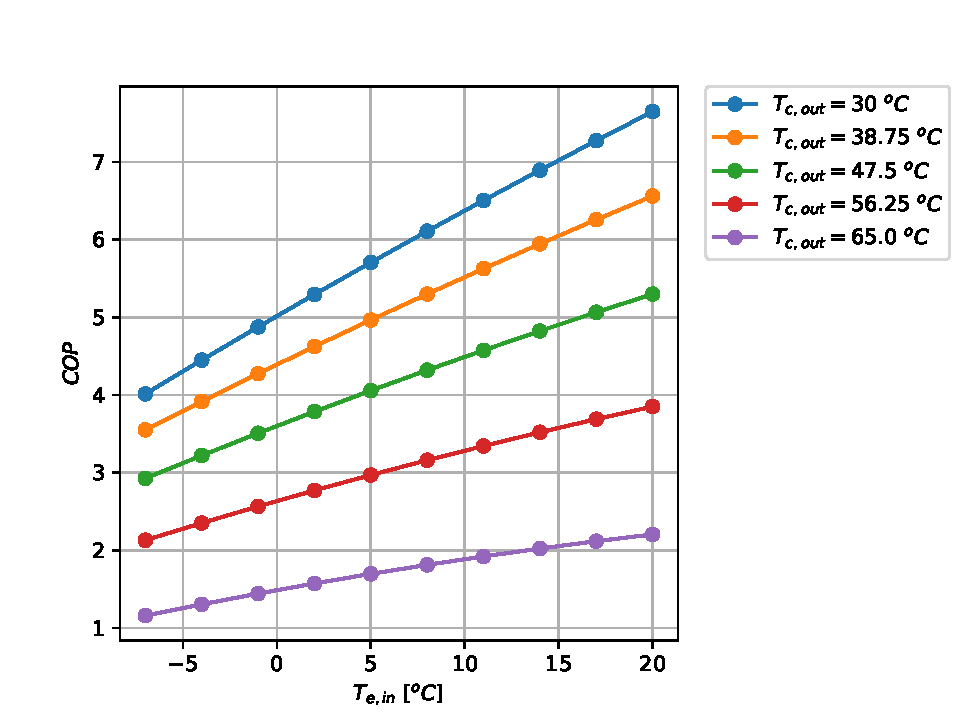
\includegraphics[width=1\textwidth]{C:/Daten/spfPackages/GIT/spfTrnsysFiles/HeatPump/BrineToWater/Walter Meier/SIN-6TU/SIN-6TU-Cop.pdf}
\caption{COP Results for the heat pump at the selected points}
\label{COPFig}
\end{center}
\end{figure}
\begin{figure}[!ht]
\begin{center}
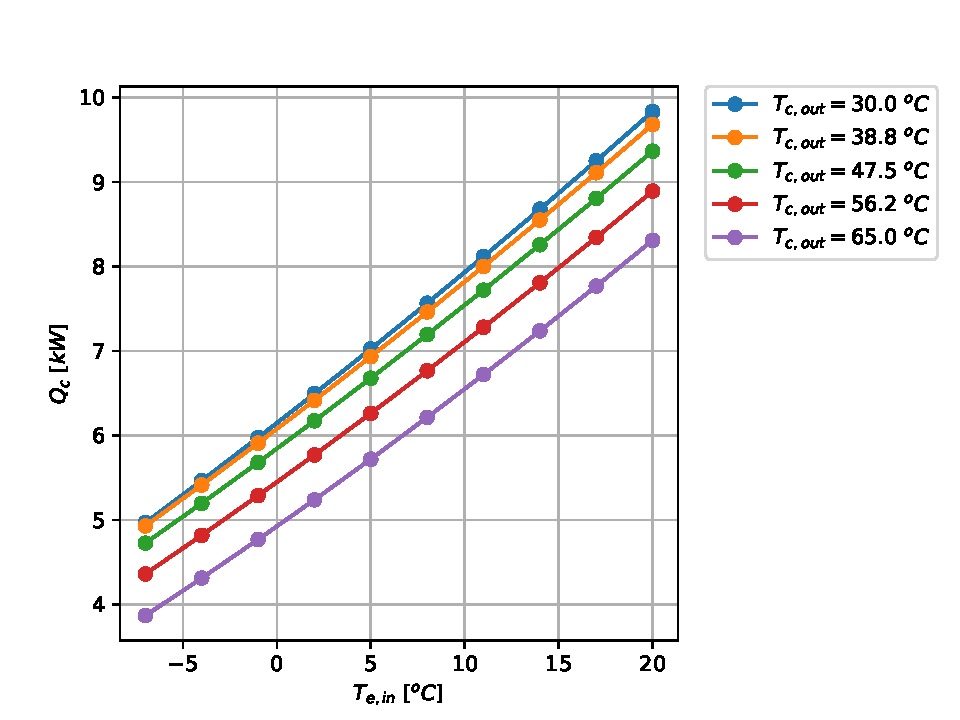
\includegraphics[width=1\textwidth]{C:/Daten/spfPackages/GIT/spfTrnsysFiles/HeatPump/BrineToWater/Walter Meier/SIN-6TU/SIN-6TU-Qc.pdf}
\caption{$Q_c$ Results for the heat pump at the selected points}
\label{QcFig}
\end{center}
\end{figure}
\end{document}
